


%%%%%%%%%%%%%%%%%%%%%%%%%%%%%%%%%%%%%%%%%%%%%%%%%%%%%%%%%%%%%%%%%%%%%%%%%%%%%%%%
%%%%%%%%%%%%%%%%%%%%%%%%%%%%%%%%%%%%%%%%%%%%%%%%%%%%%%%%%%%%%%%%%%%%%%%%%%%%%%%%
\section{\textcolor{red}{Dançar na melodia}}
\label{subsec:dancamelodia}
\index{Musicalidade!Dançar na melodia}

Como já temos visto ate agora sobre os estágios da musicalidade, 
podemos \hyperref[subsec:dancametrica]{\textbf{dançar na métrica}}  ou \hyperref[subsec:dancaritmo]{\textbf{dançar no ritmo}};
porem, quando escutamos uma música percebemos que esta não só contem ritmos estruturados, 
seguindo um acento \hyperref[def:Metrica]{\textbf{métrico}} com um \hyperref[sec:pos:timbre]{\textbf{timbre}} 
e uma \hyperref[sec:pos:Intensidade]{\textbf{intensidade}};
se não que também contem \hyperref[sec:pos:Melodia]{\textbf{melodias}} que são compostas, além de outros fatores, 
por mudanças de tons.
Conhecendo isto, 
podemos deduzir que para extrair mais atributos da música,
cuja interpretação nos leve a atingir diferentes estilos de dança,
podemos também nos concentrar no aproveitamento da melodia.


Porem, quando escutamos falar sobre dançar na melodia,
as pessoas não se referem geralmente a dançar interpretando as duas principais características de uma melodia,
que são as mudanças de \hyperref[sec:pos:Altura]{\textbf{tom}} e de
\hyperref[sec:pos:Duracion]{\textbf{duração}} nas figuras musicais;
e sim em interpretar estruturas ou aspectos mais complexos da melodia.


\begin{example}[Percebendo e estudando um poema:]
Para entender um poema poderíamos nos concentrar em estudar as letras, 
espaços em branco  e a posição destes no texto;
porem, estudar desta forma pode ser complexo para um ser humano,
que está acostumado a trabalhar pensando em macro estruturas e não em micro estruturas;
claro que a possibilidade de estudar um poema letra a letra existe,
porem não é isso o que a gente indica quando diz que quer estudar uma poesia.
Na forma mais mecânica, 
as pessoas poderiam se referir a estudar as palavras, as frases e sua função no texto;
também a forma em que as frases finalizam em rimas, a métrica,
a velocidade de leitura, entre outros fatores.
Além desta aproximação mais mecânica, 
poderíamos ascender na escala de complexidade e estudar formas ainda superiores de entender a poesia;
por exemplo, baseando-nos em aspectos mais subjetivos como, 
as emoções e sentimentos  que o texto desencadeia em nós;
ou tambem poderiamos estudar como o texto aumente e diminui a tensão em nós,
 com o uso adequado das palavras.
\end{example}

Da mesma forma que quando uma pessoa diz que vai estudar um poema, 
não se refere geralmente a estudar ela letra a letra;
quando indicamos que dançaremos na melodia,
não nos referiremos diretamente a dançar as mudanças de tom, 
e sim geralmente, se nossa visão da melodia é mais mecânica, a dançar interpretando os motivos, as frases,
o fraseio, as articulações, as cadencias, as formas estruturais, etc.
Por outro lado se procuramos uma visão e analises mais intimo da melodia,
poderíamos nos referir a interpretar com nossos movimentos, as emoções e sentimentos que a música acorda em nós;
ou poderíamos interpretar a tensão e relaxação que a melodia nos provoca,
também poderíamos incorporar na nossa dança o grau de fluidez ou descontinuidade na articulação das notas musicais, etc.

Assim, observamos que temos vários níveis, 
de onde poderemos extrair caracteristicas da melodia que possam ser interpretados em nossos movimentos;
a Figura \ref{fig:etapa-melodica-1} mostra de forma ordenada,
algumas características que podem ser extraídas da música, 
agrupados desde estruturas mais complexas (esquerda) a menos complexas (direita).
É importante ressaltar que alguns elementos destes grupos excedem a definição de melodia, como a textura, a harmonia, etc.
Estos aspectos serão tratados quando falemos sobre \hyperref[subsec:dancamusica]{\textbf{dançar na música}}.

\begin{figure}[!h]
    \centering
    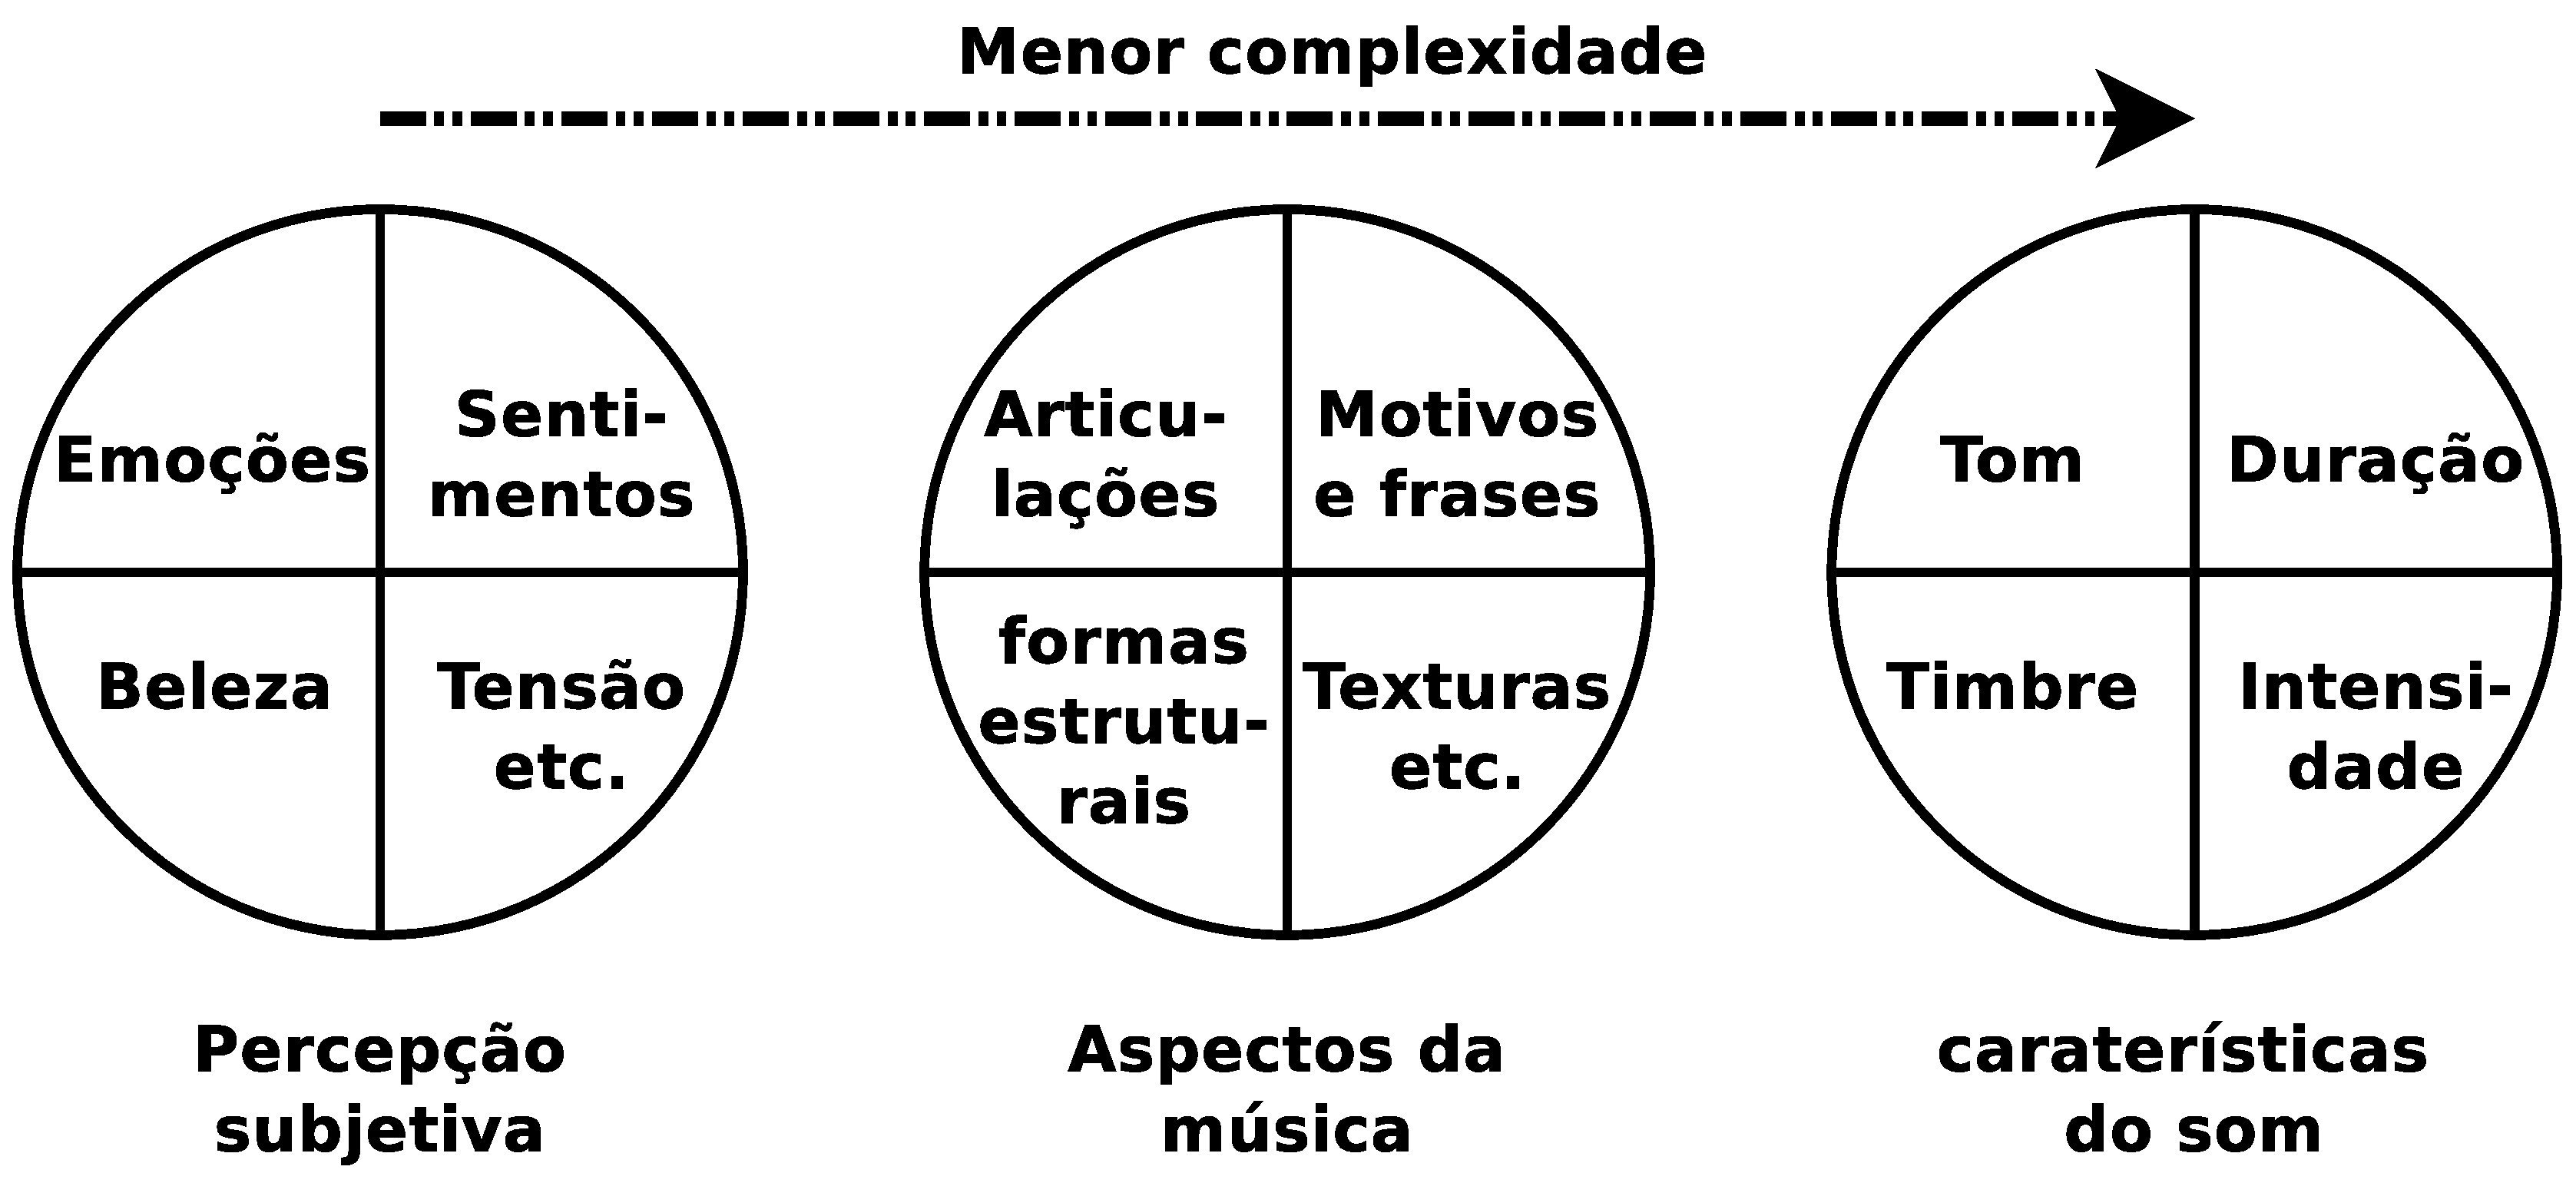
\includegraphics[width=\textwidth]{chapters/cap-musicalidade-tecnica/etapa-melodica-1.eps}
    \caption{Níveis de aproximação à música.}
    \label{fig:etapa-melodica-1}
\end{figure}

A continuação descreveremos como abordar na nossa dança o uso de uma melodia,
em todos os níveis de aproximação à música mostrados na Figura \ref{fig:etapa-melodica-1}.

%%%%%%%%%%%%%%%%%%%%%%%%%%%%%%%%%%%%%%%%%%%%%%%%%%%%%%%%%%%%%%%%%%%%%%%%%%%%%%%%
\subsection{Caraterísticas do som na melodia} 
Na 
Seção \ref{sec:elementosmusica} estudamos as \hyperref[sec:carateristasom]{\textbf{4 características do som}};
a nível de estudo da musicalidade, 
3 destas características já foram aproveitadas quando definimos \hyperref[subsec:dancaritmo]{\textbf{dançar no ritmo}};
sendo estas: 
\hyperref[sec:pos:Duracion]{\textbf{duração}}, 
\hyperref[sec:pos:Intensidade]{\textbf{intensidade}} e 
\hyperref[sec:pos:timbre]{\textbf{timbre}};
pelo que o aproveitamento destas caraterísticas não será descrito aqui\footnote{\label{footn:melodiatemritmo}Dançar 
na melodia envolve também \hyperref[subsec:dancaritmo]{\textbf{dançar no ritmo}}, 
pois toda melodia tem ritmo; 
porem, nesta seção quando falemos de dançar na melodia, 
só serão abordados aspectos da musicalidade não tratados em estagios anteriores.}.
A este nível de complexidade a única caraterística não usada é 
\{o \hyperref[sec:pos:Altura]{\textbf{tom}}\},
ou mais especificamente a mudança de \hyperref[sec:pos:Altura]{\textbf{alturas}} nas figuras musicais.

Porem, neste ponto devemos ter cuidado, 
pois seguir literalmente as mudanças de tom (altura)
seria mais próximo a \hyperref[subsubsec:musicvisualization]{\textbf{visualização musical}},
 ou a \hyperref[sec:mikeymousing]{\textbf{mickey mousing}}\footnote{Técnicas 
muito boas porem muito fáceis de virar enjoativas se são empregadas desnecessariamente.}.


\begin{example}[Seguindo o tom:] 
\label{ex:musicalidade:melodia:dtons}
Para interpretar as mudanças de tom, 
poderíamos realizar um movimento relativo\footnote{É usada a palavra ``relativo'',
pois não tem necessariamente que ser um movimento ascendente para representar um aumento de tom;
e sim, podemos digerir a ideia e mapear algum outro movimento; 
como por exemplo ir aos lados com movimentos longos.} 
a subir quando o tom aumenta,
e um relativo a descer quando o tom diminui.
\end{example}

Tecnicamente falando, 
fazer um hipotético e literal sobe e desce no Exemplo \ref{ex:musicalidade:melodia:dtons}, 
seria sim dançar na melodia\footnote{Seguir o as mudanças de tom com o corpo, 
de forma literal em todo momento, 
pode levar muito possivelmente a ter uma dança a principio engraçada e logo enjoativa.};
porem, 
existem outras caraterísticas relativas a mudanças de tom na melodia que podemos aproveitar. 

Como já foi estudado da Seção \ref{sec:caracteristicas:melodia},
podemos extrair pelo menos 3 características da melodia,
se analisamos esta em função das mudanças de tom;
estas caraterísticas são:
\{Extensão, Contorno, Movimento\}.
 
\begin{itemize}
\item \textbf{Dançando usando a extensão melódica:}
Melodias com uma \hyperref[ref:melodica:range]{\textbf{extensão melódica}} 
pequena nos produzem geralmente um clima de calma ou quietude;
por outro lado extensões maiores nos produzem geralmente uma sensação de liberdade e expansividade
 \cite[pp. 43]{holland2013music}.
Pelo que, para estar em comunião com a melodia, nossos movimentos deveriam acompanhar estas percepções.
\begin{example}[Usando o rango melódico:]
Na composição musical titulada ``Corcovado''  de Antônio Carlos Jobim,
podemos observar que esta tem uma forma $ABAC$\footnote{Com uma coda de 3 ou 4 compassos, dependendo da versão.},
com seções de 8 compassos binários cada um \cite{partituracorcovado1} \cite[pp. 53]{colluraimprovisacao}.

Ao escutar esta melodia, percebemos que as seções $A$ e $B$ tem uma extensão melódica pequena,
em comparação a seção $C$ que tem uma extensão melódica maior. 
Podemos identificar facilmente a seção $C$, pois a letra que acompanha a seção diz:
``E eu que era triste, descrente desse mundo, ao encontrar você eu conheci ...''.

Assim uma sugestão de interpretação, 
poderia ser usar movimentos com uma extensão pequena e contida para
a seção $A$ e $B$; e movimentos de percorrido mais amplo na seção $C$. 
\end{example}
\item \textbf{Dançando usando o contorno melódico:}
Quando conseguimos perceber o \hyperref[ref:melodica:shape]{\textbf{contorno}} de uma melodia,
podemos usar esta informação para visualizar mentalmente uma curva $f(t)$, em função do tempo $(t)$;
assim, podemos atrelar $f(t)$ a algum movimento ou \hyperref[sec:musicalidade:dinamicas]{\textbf{dinâmica}}.
\begin{example}[Usando a curva $f(t)$:]
Como já foi adiantado no Exemplo \ref{ex:musicalidade:melodia:dtons},
 os valores $f(t)$ podem ser usado em nossos movimentos; 
a continuação listamos algumas alternativas de uso.
\begin{itemize}
\item Distancia percorrida no salão em função de $f(t)$.
\item O espaço ocupado por nosso corpo ao realizar nossos movimentos em função de $f(t)$.
Por exemplo, se este valor é alto usamos um movimento que expanda as pernas como um ``Romário'',
ou um que expanda o espaço do \hyperref[def:Par]{\textbf{par de dança}}, como no ``assalto'', 
e se o valor de $f(t)$ é pequeno poderíamos usar movimentos no lugar usando um 
\hyperref[def:abracodedanca]{\textbf{abraço de dança}} fechado. 
\item \hyperref[subsec:dinamica:velocidade]{\textbf{Velocidade}} de nossos movimentos em função de $f(t)$.
\item \hyperref[sec:musicalidadetensionrelease]{\textbf{Tensão e relaxação}} de nosso corpo em função de $f(t)$.
\item etc.
\end{itemize}

Além de todas estas possibilidades, poderíamos fazer combinações e intercalar ou uso  destas escolhas.
\end{example}

\item \textbf{Dançando usando o movimento melódico:}
Quando vimos o tema da \hyperref[ref:melodica:range]{\textbf{extensão melódica}},
quantificamos às melodias em função da distancia entre a nota musical mais alta e a mais baixa;
este critério nos deu a possibilidade de projetar nossa dança entre dois extremos,
livre e contido, respetivamente;
porem este tipo de avaliação é um parecer promédio,
para a melodia ou uma porção dela. 
Assim, se escolhemos um movimento como deslocar-nos numa direção 
para interpretar a \hyperref[ref:melodica:range]{\textbf{extensão melódica}} numa porção de melodia,
observaremos que precisamos de um critério que nos indique como serão os sub-movimentos para completar esta ação;
este critério pode ser completado se usamos o analises do \hyperref[ref:melodica:movimento]{\textbf{movimento melódico}},
para escolher as dinâmicas dos submovimentos.
\begin{example}[Usando o movimento melódico:]
Se percebemos que a melodia esta composta por movimentos melódicos conjuntos;
então, 
os sub-movimentos de nossa dança poderiam ser executados realizando mudanças pequenas ou deslocamentos curtos,
por outro lado se percebemos movimentos melódicos disjuntos,
os sub-movimentos de nossa dança poderiam ser executados realizando mudanças grandes ou deslocamentos longos.
\end{example}
\end{itemize}


%%%%%%%%%%%%%%%%%%%%%%%%%%%%%%%%%%%%%%%%%%%%%%%%%%%%%%%%%%%%%%%%%%%%%%%%%%%%%%%%
\subsection{Aspectos da música na melodia} 
Quando analisamos a música desde um ponto de vista mais técnico, 
podemos extrair desta varias caraterísticas; 
neste sentido, nos Capítulos \ref{cap:musicabasica},
\ref{cap:musicacomposer} e \ref{cap:musicatopicos},
foram apresentadas algumas características da música, 
descritas desde o ponto de vista do compositor musical;
por outro lado, no Capítulo \ref{cap:percepcaomusical} 
foram abordados alguns aspectos da música desde o ponto de vista da percepção de um ouvinte.
Assim, juntando estas duas visões da música,
podemos formar um critério para interpretar  na nossa dança um componente da música, como a melodia.
A seguir listaremos algumas sugestões sobre escolhas criativas para interpretar a melodia na nossa dança.

Uso de dinâmicas sobre a melodia. 
\begin{itemize}
\item Motivos (leitmotiv); Uso de motivos ou ideias melódicas: Escolher um motivo, ou ideia melódica pequena e dar um passo no final, 
aplicando uma dinâmica em concordância com a ideia melódica.
\item Frases (cadências).
\item Fraseio da linha melódica.
\item Articulações
\item Formas estruturais.
\end{itemize}



%%%%%%%%%%%%%%%%%%%%%%%%%%%%%%%%%%%%%%%%%%%%%%%%%%%%%%%%%%%%%%%%%%%%%%%%%%%%%%%%
\subsection{Percepção subjetiva da melodia} 

Você precisará se concentrar na qualidade expressão emocional da linha melódica.

Melodia não pode existir sem ritmo, mas acrescenta emoção, doçura e continuidade à música.

Melodia é o que faz com que nossos passos para se tornar elegante, 
graciosa, sentimental e persistente, enquanto tentamos expressar a beleza, emoção e fluidez da melodia.


\begin{itemize}
\item eu sigo a intensidade da mesma.
\end{itemize}

%%%%%%%%%%%%%%%%%%%%%%%%%%%%%%%%%%%%%%%%%%%%%%%%%%%%%%%%%%%%%%%%%%%%%%%%%%%%%%%%
\subsection{Exemplos} 

Para darle un poco más de libertad y creatividad, 
mantener el pulso o el ritmo en sus pies le brinda la capacidad de interpretar 
la melodía con el resto de su cuerpo ou realizando dinâmicas, si así lo desea.


